\textbf{{1.UDP的基本概念}}

UDP和TCP最大的区别在于它是无连接的,UDP其实只在IP的数据报服务之上增加了端口的功能(为了找到进程)和差错检测的功能。

虽然UDP用户数据报只能提供不可靠的交付,\textbf{但UDP在某些方面有其特殊的优点。}

\textbf{1)}发送数据之前不需要建立连接\textbf{。}

\textbf{2)}UDP的主机不需要维持复杂的连接状态表。

\textbf{3)}UDP用户数据报只有8个字节的首部开销。\\

\textbf{4)}网络出现的拥塞不会使源主机的发送速率降低。

\textbf{5)}UDP支持一对一、一对多、多对一和多对多的交互通信。

\textbf{{2.UDP数据报的组成}}

UDP数据报有两个字段:数据字段和首部字段。首部字段有8B,由4个字段组成,如下图所示。

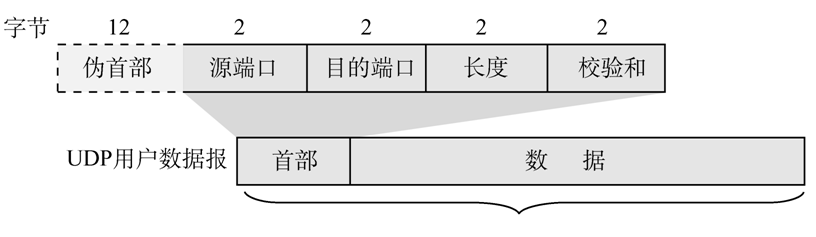
\includegraphics[width=3.12500in,height=0.90625in]{png-jpeg-pics/8BF4290E57D76DF799073EA77AC636FA.png}

\textbf{1)源端口。}占2B。前面已经说了使用16bit来表示端口号,所以需要2B长度。

\textbf{2)目的端口。}占2B。

\textbf{3)长度。}占2B。

\textbf{4)校验和。}占2B。用来检测UDP用户数据报在传输中是否有错(既检验首部,又检验数据部分),如果有错,就直接丢弃;若该字段为可选字段,当源主机不想计算校验和时,则直接令该字段为全0。\textbf{检验范围:伪首部、UDP数据报的首部和数据。其中,在计算校验和时临时生成伪首部}。
